% ----------------------------------------------------------------------- %
% Arquivo: cap2.tex
% ----------------------------------------------------------------------- %

\chapter{Arquiteturas  WEB}
\label{c_cap2}

Uma aplicação \textit{web} é um \textit{software} que roda no lado do cliente, ou seja, na máquina do próprio usuário, com essa abordagem é necessário  apenas que o cliente possua um \textit{browser}(navegador), independente de seu sistema operacional para acessar uma aplicação \textit{web}. Com isso os desenvolvedores não precisam desenvolver diversas versões de uma mesma aplicação, para sistemas operacionais diferentes.

Tendo isso em vista, este capítulo visa apresentar um breve histórico da evolução da arquitetura  \textit{web}, apresentará o modelo de multicamadas e por fim demonstrará seus estilos arquitetônicos.

\section{História}


A Internet mudou completamente quando Tim Berners-Lee, a fim de solucionar os problemas de comunicações da \ac{CERN}, propôs que se usasse um sistema de comunicação em hipertexto. Esse sistema acabou agradando os gerentes do \ac{CERN}, e no ano seguinte, ele foi implantado com o nome de \textit{\ac{WWW}}. Todos os serviços da \textit{Internet} se renderam ao poder da \textit{Web} e à linguagem \ac{HTML}, que a sustenta. Até o serviço de correio eletrônico, campeão de tráfego na \textit{Internet} por muitos anos, que por muito tempo exigia aplicações específicas, separadas do \textit{browser}, hoje é lido dentro de um \textit{browser}, através de páginas \ac{HTML} \cite{rocha99}. 

A medida que o \ac{HTML} foi ganhando fama, quem a usava não queria apenas uma simples apresentação de texto estruturada, queriam usar cores, imagens e técnicas de design mais avançado, suas páginas \ac{HTML} acabavam ficando com vários códigos de estilos. Só que a manutenção seria o maior problema dessa abordagem, se um componente mudar de estilo em apenas uma página a alteração seria simples, mas se fosse em várias páginas, a manutenção já seria bastante penosa. Misturar estilo e estrutura não era mais interessante, e foi assim que em 1995, Håkon Wium Lie e Bert Bos apresentaram a proposta do \ac{CSS} que logo foi apoiada pela \ac{W3C}. A ideia geral era, utilizar \ac{HTML} somente para estruturar o \textit{website} e a tarefa de apresentação fica com o \ac{CSS} disposto em um arquivo separado com o sufixo .css ou no próprio \ac{HTML} demarcado pelas tags <style> \cite{devmediaCSS2018}.

O ano de 1995 é muito importante para a \textit{internet}, a Netscape Communications apresenta o \textit{Javascript}, uma linguagem leve, interpretada e baseada em objetos com funções de primeira classe, mais conhecida como a linguagem de \textit{script} para páginas \textit{Web}, mas usada também em vários outros ambientes sem \textit{browser} como \textit{node.js},  \textit{Apache CouchDB} e\textit{ Adobe Acrobat}. O \textit{Javascript} é uma linguagem de script multi-paradigma,  baseada em protótipo que é dinâmica, e suporta estilos de programação orientado a objetos, imperativo e funcional \cite{mozilla2018}, e possibilitou que os desenvolvedores pudessem criar componentes dinâmicos, e assim possibilitando uma melhora na \textit{interface} do usuário. Com o \textit{javascript} a \textit{internet} acabou se tornando mais performática e produtiva, porque os dados não precisavam mais ser enviados ao servidor para se gerar toda a página \ac{HTML}. Juntos o \textit{Javascript}, \ac{HTML} e \ac{CSS} são às três tecnologias mais populares para a produção de conteúdo na internet \cite{devsaran2018}.

Já no ano de 1996 a Macromedia lançaria o \textit{Flash}, que é uma plataforma multimídia de desenvolvimento para aplicações que contenham animações, áudio e vídeo, bastante utilizada na construção de anúncios publicitários e páginas \textit{web} interativas. O \textit{Flash} pode manipular vetores e gráficos para criar textos animados, desenhos, imagens e até \textit{streaming} de áudio e vídeo pela internet. 
O \textit{Flash} ganhou bastante popularidade entre os programadores e desenvolvedores \textit{web} por permitir um desenvolvimento rápido de aplicações com alta qualidade e integração transparente com outras categorias de conteúdo \cite{canaltechFlash2018}.

 Com o \textit{Flash} os programadores puderam dar ao usuário, uma experiência mais rica através de animações de áudio e vídeo. Além disso, as interações feitas no \textit{Flash} eram todas no lado do cliente, não precisando se comunicar com o servidor. Era comum que os \textit{sites} antes dos anos 2000, usasse conteúdo multimídia incorporado, o que por muitas vezes gerava uma poluição visual muito grande, e como consequência disso a popularidade do \textit{Flash} acabou caindo, as páginas acabaram ganhando um visual padrão, o acesso do usuário não era mais interrompido por áudio, vídeos e anúncios inesperados, a medida que seu uso foi diminuindo a página ficava mais leve e o uso de rede também \cite{devmediaAsync2018}.


 Apesar de  seu uso ir diminuindo gradualmente, o \textit{Flash} por muitos anos foi usado para criação de jogos e aplicativos interativos para dispositivos móveis. No ano de 2008 o primeiro rascunho público do \ac{HTML}5 é lançado pelo \textit{WHATWG} \cite{fasthosts2018}, essa tecnologia ganhou os holofotes, foi quando em 2010 o CEO da Apple Inc., Steve Jobs emitiu uma carta pública intitulada "Reflexões sobre o Adobe Flash", onde ele conclui que o desenvolvimento do \ac{HTML}5 tornaria o \textit{Flash} não mais necessário para exibir qualquer conteúdo \textit{web}. Depois disso o fim do \textit{Flash} era questão de tempo, muitos \textit{browsers} já não o utilizavam mais, e em julho de 2017, em comunicado oficial a Adobe, anunciou que vai encerrar definitivamente o suporte para sua tecnologia Flash até 2020. A companhia disse precisar destes últimos anos para incentivar criadores de conteúdo e desenvolvedores a utilizarem novas plataformas, principalmente formatos de código aberto e que funcionem também em celulares e \textit{tablets}  \cite{canaltechFlashFim2018}.

Em 1999, o conceito de aplicação \textit{web} apareceu na linguagem Java. Mais tarde, em 2005, o Ajax foi apresentado por Jesse James Garrett em seu artigo "Ajax: uma nova abordagem para a aplicação Web". Esta nova técnica de desenvolvimento, possibilitou a criação de aplicações \textit{web} assíncronas, ou seja, o fluxo do código não é interrompido até que a resposta seja obtida. Ao invés disso, após realizar a requisição, a resposta é obtida em um momento posterior, de forma independente, e tratada por uma função (chamada função de \textit{callback}). Com isso era possível enviar dados para o servidor e recuperá-los sem interferir na navegação de uma página específica, não precisando baixar a página inteira \cite{devmediaAsync2018}.


\section{Modelo de Multicamadas}
\label{s_c2_figuras}


\subsection*{Modelo de uma camada}

Esse modelo foi fortemente usado durante os anos 1960 até meados dos anos 80, também chamado de sistemas centralizados ou de arquitetura uni processada, o modelo de uma camada era caracterizado por manter todos os recursos do sistema (banco de dados, regras de negócios e interfaces de usuário) em computadores de grande porte, os conhecidos mainframes. Os terminais clientes não possuíam recursos de armazenamento ou processamento, sendo conhecidos como terminais burros ou mudos. Nesta arquitetura, o mainframe tinha a responsabilidade de realizar todas as tarefas e processamento \cite{devmediaMultiCamada2018}. As aplicações eram escritas em um único módulo ou camada monolítica, com programas e dados firmemente entrelaçados. Tal integração estreita entre programa e dados dificultava a evolução e reuso de componentes. Cada desenvolvedor de aplicação escolhia como estruturar e armazenar os dados e usava-se frequentemente técnicas para minimizar o caro armazenamento e manipulação em memória principal \cite{devmediaMultiCamadaP12018}.


\subsection*{Modelo de duas camadas}

Também conhecido como modelo cliente-servidor, seu uso se deu bastante durantes os anos 1980 à 1990, durante essa época novas tecnologias foram desenvolvidas e adotadas como, \textit{softwares} para gerenciamento de banco de dados relacionais (SGBD), a utilização de rede locais interligando microcomputadores departamentais, o início do paradigma da programação orientada a objetos, e a redução dos custos do hardware, tornando possível a massificação da computação pessoal \cite{devmediaMultiCamadaP12018}. Também devido à grande expansão das redes de computadores, os métodos para desenvolvimento de \textit{software} foram aos poucos evoluindo para uma arquitetura descentralizada, na qual não somente o servidor era responsável pelo processamento, mas as estações clientes também assumem parte desta tarefa. Dentro deste contexto que surgiu o modelo de duas camadas, justamente com o objetivo de dividir a carga de processamento entre o servidor e as máquinas clientes \cite{devmediaMultiCamada2018}. A \autoref{f_c2_cliente_servidor}  é uma representação do modelo cliente-servidor.

\begin{figure}[h!]
\centering
\caption{Modelo Cliente-Servidor}
\frame{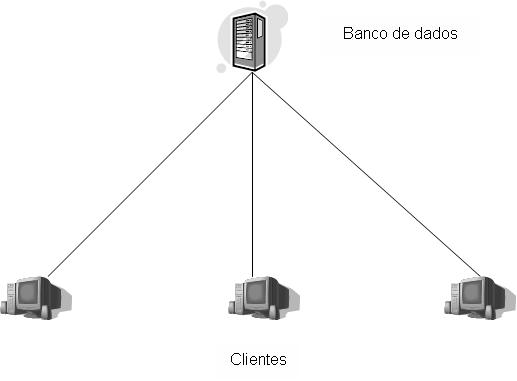
\includegraphics[scale=0.60]{images/cliente-servidor}}\\
Fonte: \cite{devmediaMultiCamadaP12018}
\label{f_c2_cliente_servidor}
\end{figure}

Na camada do cliente, é onde o usuário interage com o sistema, ela é responsável por prover uma \ac{UI} agradável e de fácil acesso para o usuário possa manipular o sistema. Mas apesar de prover a \ac{UI}, a camada do cliente não se restringe a isso, regras de negócio também podem ser implementadas, assim diminuindo a complexidade no servidor. A camada do cliente, de acordo com a sua  complexidade pode ser definida de duas formas segundo \cite{devmediaMultiCamadaP12018}. Sendo elas:

\begin{itemize}
    \item Cliente Gordo
    \begin{itemize}
        \item Maior complexidade de regras de negócio
        \item Menos processamento para o servidor
        \item Possivelmente mais tráfego na rede
        \item Cliente é mais sensível a mudanças
    \end{itemize}
    \item Cliente Magro
    \begin{itemize}
        \item Menor complexidade de regras de negócio
        \item Mais processamento para o servidor
        \item Menor tráfego na rede
        \item Manutenção mais simples
    \end{itemize}
\end{itemize}

Com o modelo de duas camadas foi possível que \textit{softwares} de terceiros tivessem acesso ao banco de dados, ou seja, com isso os \textit{softwares} poderiam ser diferentes para cada usuário ou setor, afim de melhor atender às suas necessidades. Outra vantagem é a questão do custo-beneficio, as estações dos clientes são mais baratas do que um servidor \cite{devmediaMultiCamadaP12018}.

O modelo de duas camadas também pode apresentar algumas desvantagens, como sua aplicação é dividida em partes, acaba acarretando em um \textit{software} mais complexo, com novos cenários a serem tratados. A comunicação do cliente com o servidor se dá por meio da rede, com isso dados sensíveis serão trafegados na rede e precisam de um cuidado maior com a criptografia \cite{rocha99}. 

\subsection*{Modelo de Multicamadas}
Modelo de multicamadas ou cliente servidor de múltiplas camadas, se consolida a partir dos anos 90 como resposta a  popularização da internet e melhoria das tecnologias de redes, sendo  uma evolução do modelo de duas camadas. Ele tem como propósito  que uma aplicação cliente não realizasse comunicação direta com o banco de dados, no meio do caminho haveria uma ou mais camadas, que elas sim se comunicariam com o banco de dados. A ideia básica é distribuir o processamento da aplicação em várias máquinas, evitando a sobrecarga sobre uma única camada, como ocorria no modelo cliente-servidor. Com a distribuição da carga de processamento em diversas máquinas é possível melhorar o desempenho e compartilhar recursos, utilizando-os como se fossem recursos locais, característica conhecida como  transparência de uso \cite{devmediaMultiCamadaP12018}. Com isso a aplicação pode ser dividida em pequenos pedaços, cada um com sua responsabilidade. Além dessas vantagens, há uma compensação no custo em relação ao desempenho, a possibilidade de aumento de escala e expansão da rede sem perda de qualidade, melhora na robustez em função da distribuição dos serviços em mais de uma máquina, e muitos outros benefícios \cite{devmediaMultiCamadaP12018}.

Em uma aplicação que faz uso do  modelo de multicamadas, faz se necessário ao menos três camadas: camada de apresentação, camada de regras de negócio e a camada de dados. A \autoref{f_c2_multicamada} apresenta o esquema de um sistema multicamada. 

\begin{figure}[!htpb]
	\centering
	\caption{Modelo Multicamada}
	\label{f_c2_multicamada}
	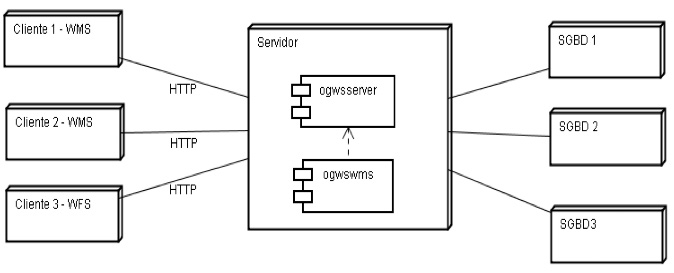
\includegraphics[width=14cm]{images/multicamada.jpg}\\
    Fonte: \cite{diegomacedoArqApp}
 
\end{figure}

\subsection{Camada de Apresentação}

A camada de apresentação fica fisicamente localizada na estação cliente e é responsável por fazer a interação do usuário com o sistema. É uma camada bastante leve, que basicamente executa os tratamentos de telas e campos e geralmente acessa somente a segunda camada, a qual faz as requisições ao banco de dados e devolve o resultado. É também conhecida como cliente, regras de interface de usuário ou camada de interface \cite{devmediaMultiCamada2018}.

\subsection{Camada de Regra de Negócio}

Também conhecida como servidor de aplicação, lógica de negócio ou camada de acesso a dados, essa camada é a responsável por intermediar a comunicação entre a camada de apresentação com a camada de dados, só ela tem acesso a camada de dados. O servidor de aplicação é, geralmente, uma máquina dedicada e com elevados recursos de hardware, uma vez que nele é que ficam armazenados os métodos remotos (regras de negócios) e é realizado todo o seu tratamento e processamento. \cite{devmediaMultiCamada2018}.

\subsection{Camada de Dados}

Também chamada de camada de banco de dados, essa camada é onde se localiza o \ac{SGBD}, ela é responsável por receber requisições da camada de regra de negócio, interpretá las e assim executá-las no banco de dados  \cite{devmediaMultiCamada2018}.


\section{Vantagens}

O modelo de multicamadas apresentou diversas vantagens em relação ao modelo de duas camadas, são essas as que mais se destacam:

\subsection{Clientes Leves}

Diferentemente do modelo de duas camadas, onde a regra de negócio era divida tanto na camada do cliente quanto na do servidor, aqui a camada intermediária é quem fica a cargo disso, na camada de apresentação será apenas para visualização de dados, além de possuir possíveis tratamentos de campos e telas  \cite{devmediaMultiCamada2018}.

\subsection{Facilidade de Redistribuição}

As estações clientes acessam a mesma camada intermediária, sendo assim, quando houver novas implementações ou alterações nas regras de negócios, será refletido para todas as estações clientes  \cite{devmediaMultiCamada2018}.

\subsection{Modularização}

A modularização refere-se a separar a lógica do negócio e regras de acesso ao banco de dados da camada de apresentação. Desta maneira, várias aplicações clientes podem compartilhar as mesmas regras, que ficam encapsuladas em uma camada de acesso comum.Assim sendo, as regras ficam centralizadas em um único local, ao contrário de em uma aplicação desenvolvida em duas camadas, na qual geralmente existe redundância nestas regras e uma mudança mesmo que pequena acarretará na redistribuição do aplicativo em cada estação cliente \cite{devmediaMultiCamada2018}.

\subsection{Economia de conexões no servidor}

Em um sistema com o modelo de duas camadas, as estações clientes se comunicavam diretamente ao servidor que se localizava o banco de dados, então para cada estação cliente conectada era uma conexão aberta com o banco de dados, sendo que o banco de dados possuí um limite para conexões, tendo isso em vista, no modelo de multicamadas isso não ocorre já que quem se conecta com o banco de dados é o servidor de aplicação, localizado em uma camada intermediária, e uma conexão realizada pelo servidor de aplicação é compartilhada para as estações clientes a ele conectado, sendo assim poderia se ter várias estações clientes requisitando recursos do banco de dados, mas apenas uma conexão estaria aberta já que quem ficaria responsável pela conexão é o servidor de aplicação \cite{devmediaMultiCamada2018}.

\subsection{Independência de localização}

A localização não é um empecilho para a comunicação entre camadas, a estação cliente pode estar fisicamente distante para acessar as camadas intermediárias  \cite{devmediaMultiCamada2018}.

\subsection{Escalabilidade}

No modelo de duas camadas, quando um grande número de estações clientes se conectam ao servidor, acaba ocorrendo uma grande perda de desempenho. Já com o modelo de multicamadas este problema pode ser contornado, já que é possível replicar a regra de negócio em servidores distintos através do balanceamento de carga, isso quer dizer que quando um servidor de aplicação estiver sobrecarregado, outro servidor é acionado para ajudar no controle de conexões, isso também pode ser usado quando um servidor de aplicação parar de funcionar \cite{devmediaMultiCamada2018}.

\section{Estilos Arquitetônicos}

Nesta seção será apresentados os estilos arquitetônicos de desenvolvimento de uma aplicação web.

\subsection{Arquitetura Monolítica}

Segundo \cite{monoVsMicro2017},  "Uma aplicação monolítica é aquele tipo de aplicação na qual toda a base de código está contida em um só lugar, ou seja, todas as funcionalidades estão definidas no mesmo bloco". Esse bloco geralmente se divide em três partes: apresentação, negócio e dados. A \autoref{f_c2_app_monolitica} apresenta o modelo dessa arquitetura.

\begin{figure}[h]
	\centering
	\caption{Aplicação Monolitica}
	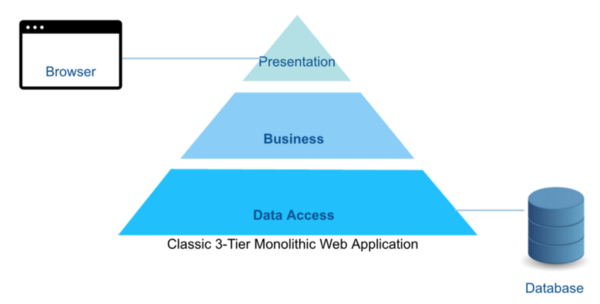
\includegraphics[scale=0.7]{images/app-monolitica.png}\\
	Fonte:\cite{monoVsMicro2017}
 	\label{f_c2_app_monolitica}
\end{figure}

\newpage
\subsection*{Camadas}

\subsection*{Apresentação}
Camada responsável pela visualização ou interface, que será apresentada para o usuário. "Em uma aplicação web, esta camada contém as páginas \ac{HTML} com \ac{JS} e \ac{CSS} que serão renderizadas no \textit{browser} de quem as acessar",  \cite{monoVsMicro2017}.

\subsection*{Negócio}
Camada que é responsável pela lógica da aplicação. Segundo \cite{monoVsMicro2017} "Nesta camada geralmente se encontram todas as bases de código, chamadas, \ac{API}'s e literalmente toda a inteligência do sistema em questão".

\subsection*{Dados}
Camada em que se encontram as classes encarregadas pela conexão com o \ac{SGBD} ou outro tipo de sistema de armazenamento de dados \cite{monoVsMicro2017}.

\subsection*{Vantagens}
\begin{itemize}
	\item Fácil deploy da aplicação.
	\item Não há duplicidade de código.
	\item Aplicação é desenvolvida usando uma mesma tecnologia.
	\item Seu desenvolvimento tende a ser mais rápido, por ser uma arquitetura mais simples.
	\item Fluxo de deploy simples.
\end{itemize}

\subsection*{Desvantagens}
\begin{itemize}
	\item Ponto único de falha.
	\item Aumento de tamanho e complexidade ao longo do tempo.
	\item Falta de flexibilidade, já que usa uma mesma tecnologia.
	\item Baixa escalabilidade, tendo que copiar toda a aplicação para escalar horizontalmente.
	\item Alta dependência de componentes.
	\item Dificuldade de alterações em produção, qualquer mudança se faz necessário, a reinicialização de todo o sistema.
	\item Demora de aculturamento, um novo desenvolvedor pode ter dificuldades para entender o funcionamento de um componente.
\end{itemize}

\subsection{Arquitetura de Micro serviços}
Uma arquitetura de micro serviços segundo \cite{microservices2014}:  \begin{citacao}"é uma abordagem que desenvolve uma aplicação única como uma suíte de pequenos serviços, cada um rodando em seu próprio processo e se comunicando com mecanismos leves, geralmente uma \ac{API} de recurso \ac{HTTP}" \end{citacao} Desse jeito nós separamos uma aplicação monolítica em pequenas aplicações autônomas, ou seja, devem possuir um sistema de deploy automático e independente, além de que cada aplicação possui um conjunto de regras de negócio específico. A \autoref{f_c2_app_monolitica_vs_microservices} mostra a comparação entre a arquitetura monolítica e de micro serviços.



\begin{figure}[!htpb]
	\centering
	\caption{Representação de módulos monolítico e micro serviços}
	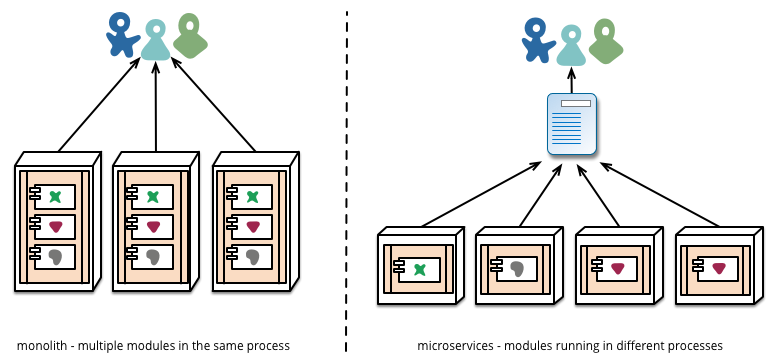
\includegraphics[width=15cm]{images/micro-deployment.png}\\
	Fonte: \cite{microservices2014}
 	\label{f_c2_app_monolitica_vs_microservices}
\end{figure}

\subsection*{Vantagens}
\begin{itemize}
	\item Arquitetura individual simples.
	\item Sistemas totalmente independentes.
	\item Ausência de ponto de falha única.
	\item Fácil deploy da aplicação e testes unitários.
	\item Módulos podem usar tecnologias distintas.
	\item Serviços coesos e desacoplados.
	\item Facilidade de alterações em ambiente de produção, apenas o serviço específico é necessário ser reinicializado para refletir as alterações.
	\item Escalabilidade do sistema, serviços que sofrem de alta demanda podem ser replicados individualmente.
\end{itemize}

\subsection*{Desvantagens}
\begin{itemize}
	\item Desempenho prejudicado pela latência da rede e pelo custo de serialização e deserialização.
	\item Se a aplicação não for bem documentada, a arquitetura geral tende a ser tornar complexa.
	\item Falta de planejamento e má execução, a arquitetura pode se tornar uma grande bagunça.
	\item Repetição de código nos serviços.
\end{itemize}

